% Slide Designed by 
% Hazoor Ahmad
% PhD Electrical Engineering
% Vision Processing Lab, (VISPro),
% Information Technology University, Lahore

\documentclass{beamer}
\renewcommand{\baselinestretch}{1.5} 
\usepackage{cite}
\usepackage{amsmath,amssymb,amsfonts}
\usepackage{algorithmic}
\usepackage{graphicx}
\usepackage{diagbox}
\usepackage{array,multirow}


\usepackage{hyperref}
\hypersetup{
	pdftitle={Thesis Presentation By Hazoor Ahmad PhDEE17004},
   colorlinks=true,
   citecolor=blue,
   linkcolor=blue,
   urlcolor=blue
}

\usefonttheme{structurebold}
\setbeamercolor{title}{fg=black}
\setbeamercolor{frametitle}{fg=black}
\setbeamercolor{structure}{fg=black}

\title{Interconexión del robot NAO a servicios de simulación en la nube}
\author{Hazoor Ahmad}
\date{}
\addtobeamertemplate{navigation symbols}{}{%
    \usebeamerfont{footline}%
    \usebeamercolor[fg]{footline}%
    \hspace{1em}%
    \insertframenumber/\inserttotalframenumber
}
\definecolor{blue(pigment)}{rgb}{0.2, 0.2, 0.6}
\def\bsq{\color{blue(pigment)} $\blacksquare$ \color{black}}
\begin{document}
% Set Title Slide Background Here
\usebackgroundtemplate{\includegraphics[width=\paperwidth, height=\paperheight]{Title_Slide_bg.pdf}}
\frame{\titlepage}
% Set Other all Silde Background Here
\usebackgroundtemplate{\includegraphics[width=\paperwidth, height=\paperheight]{Other_Slides_bg.pdf}}

% Slide 1
\begin{frame}{Myself\\\rule{10.5cm}{0.5pt}} \label{slide1}
\bsq The Overview is given at Slide ~\ref{overview}\\
\bsq This is a test page! \\
\bsq This is a test page! \\
\bsq This is a test page! \\
\bsq This is a test page! \\
\bsq This is a test page! \\
\bsq This is a test page!
\end{frame} 

% Slide 2 : showing eps file from matlab/octave
\begin{frame}{Overview\\\rule{10.5cm}{0.5pt}} \label{slide2}
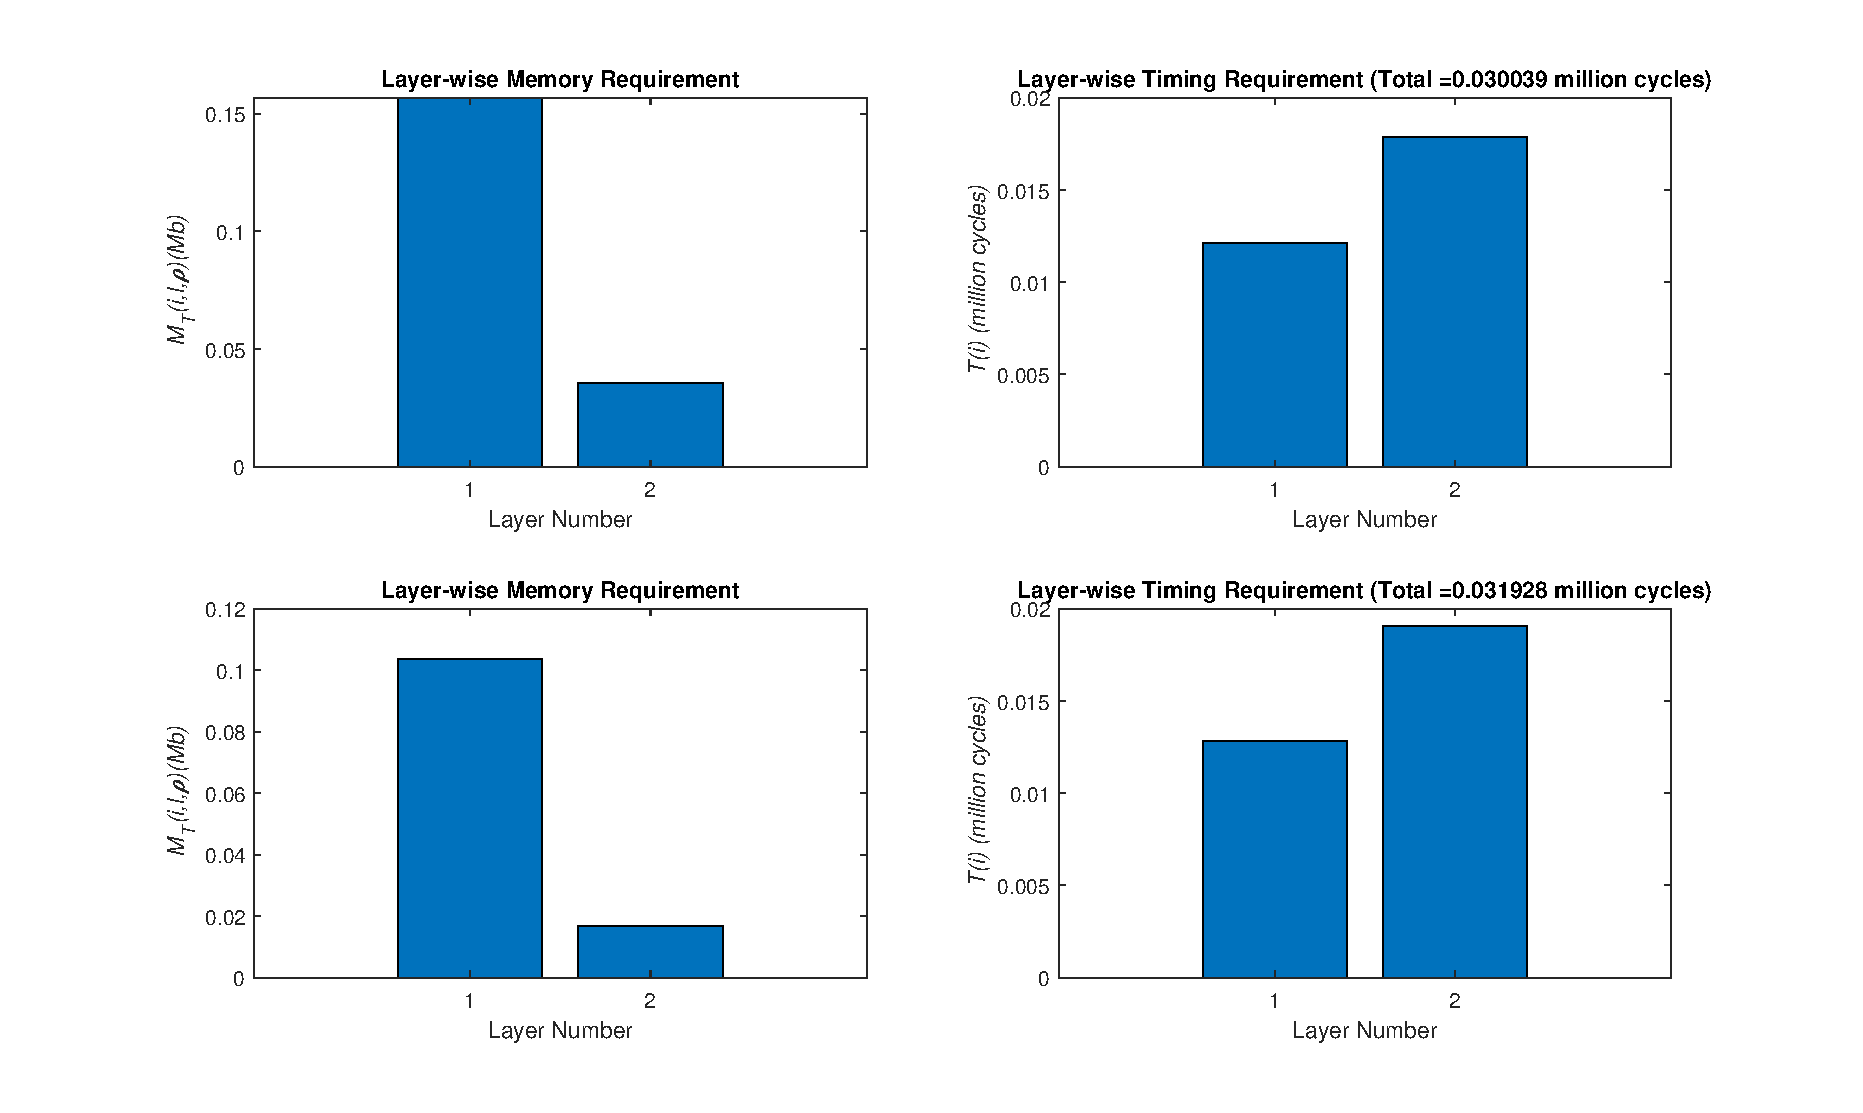
\includegraphics[width=0.8\paperwidth]{overview.eps}
\end{frame}

% Slide 3
\begin{frame}{Introduction\\\rule{10.5cm}{0.5pt}} \label{slide3}
\bsq This is a test page! \\
\bsq This is a test page! \\
\bsq This is a test page! \\
\bsq This is a test page! \\
\bsq This is a test page! \\
\bsq This is a test page!
\end{frame}

% Slide 4 : showing pdf file from power point/ corel draw / inkscape etc
\begin{frame}{Explanation of a Code Segment from 2D Convolution using Vivado HLS\\\rule{10.5cm}{0.5pt}} \label{slide4}
\includegraphics[trim=10 15 50 80,clip,width=0.9\paperwidth]{pdf_file.pdf} % Crop image [trim =  <left><bottom><right><top>]
\end{frame}

% Slide x : Plan slide
\begin{frame}{Overview\\\rule{10.5cm}{0.5pt}} \label{overview}

\begin{table}
\begin{tiny}
\renewcommand{\arraystretch}{0.4}
\begin{tabular}{|p{3.7cm}||m{0.4cm}|m{0.4cm}|m{0.4cm}|m{0.4cm}|m{0.4cm}|m{0.4cm}|}
\hline \backslashbox[4cm]{\textbf{Activity}}{\textbf{Time}}&\textbf{F18}&\textbf{S19}&\textbf{F19}&\textbf{S20}&\textbf{F20}&\textbf{S21}\\
\hline 
\hline Literature Review and Study          &\begin{center}{\checkmark} \end{center}     &&&&&\\ [-0.2cm]
\hline Analysis and Design of Techniques    &&\begin{center}{\checkmark} \end{center}     &&&&\\ [-0.2cm]
\hline FPGA Implementation                  &&&\begin{center}{\checkmark} \end{center}     &&&\\ [-0.2cm]
\hline Final Results \& Optimization        &&&&\begin{center}{\checkmark} \end{center}     &&\\ [-0.2cm]
\hline Thesis Writing \& Publication        &&&&&\begin{center}{\checkmark} \end{center}     &\\ [-0.2cm]
\hline External Review \& Final Defense     &&&&&&\begin{center}{\checkmark} \end{center}     \\ [-0.2cm]
\hline \\\hline
\end{tabular}
\label{gantt}
\end{tiny}
\end{table}
\end{frame}


% Slide x : Last Slide
\begin{frame} \label{lastslide}
\begin{center}
{\fontsize{40}{50}\selectfont Thank You!}
\end{center}
\end{frame}


\end{document}